% ==============================================================================
% Section VII: Multiplier-Free Polynomial Codecs & Serialization Architecture
% IEEE Transactions on VLSI Systems / Information Forensics & Security
% ==============================================================================

\section{Multiplier-Free Polynomial Codecs and Serialization Architecture}
\label{sec:poly_codecs}

Polynomial coefficient compression, decompression, and byte serialization constitute the operational boundary between high-dimensional ring arithmetic and external communications in the Module-Lattice-Based Key-Encapsulation Mechanism (\mbox{ML-KEM}), standardized in NIST FIPS~203~\cite{fips203}. Unlike classical public-key cryptosystems whose boundary encodings are simple bitwise concatenations or power-of-two byte packings, \mbox{ML-KEM} mandates lossy mathematical compression functions involving non-power-of-two modular divisions and half-integer round-to-nearest arithmetic across multiple dynamically selected bit-depths. Furthermore, public keys, secret keys, and ciphertexts must be converted between vectors of 12-bit ring coefficients in $\mathcal{R}_q = \mathbb{Z}_q[X]/(X^{256} + 1)$ with prime modulus $q = 3329$ and packed byte streams.

In conventional post-quantum cryptographic (PQC) hardware designs, these codec operations introduce substantial latency overheads, consume disproportionate DSP multiplier slices or multi-cycle hardware division IPs, and instantiate complex variable-length dynamic barrel shifters whose multi-level multiplexer trees restrict overall operating frequencies~\cite{xing2023tcas1, imran2022tvlsi}. In this section, we present the microarchitecture of the polynomial codec and serialization subsystem developed for the proposed accelerator. By exploiting fixed-point Canonical Signed Digit (CSD) scaling, balanced modulus decomposition, dual-bank ping-pong buffering governed by 8-coefficient chunk byte alignment, and static bit-slice multiplexer trees, the subsystem completely eliminates hardware dividers, dedicated DSP blocks, and dynamic barrel shifters while sustaining continuous wire-speed throughput at 480+~MHz standalone and 413.7~MHz when fully integrated into the top-level core.

The complete microarchitectural topology of the polynomial codec subsystem is depicted in Fig.~\ref{fig:poly_codecs_compress}.

\begin{figure*}[!t]
\centering
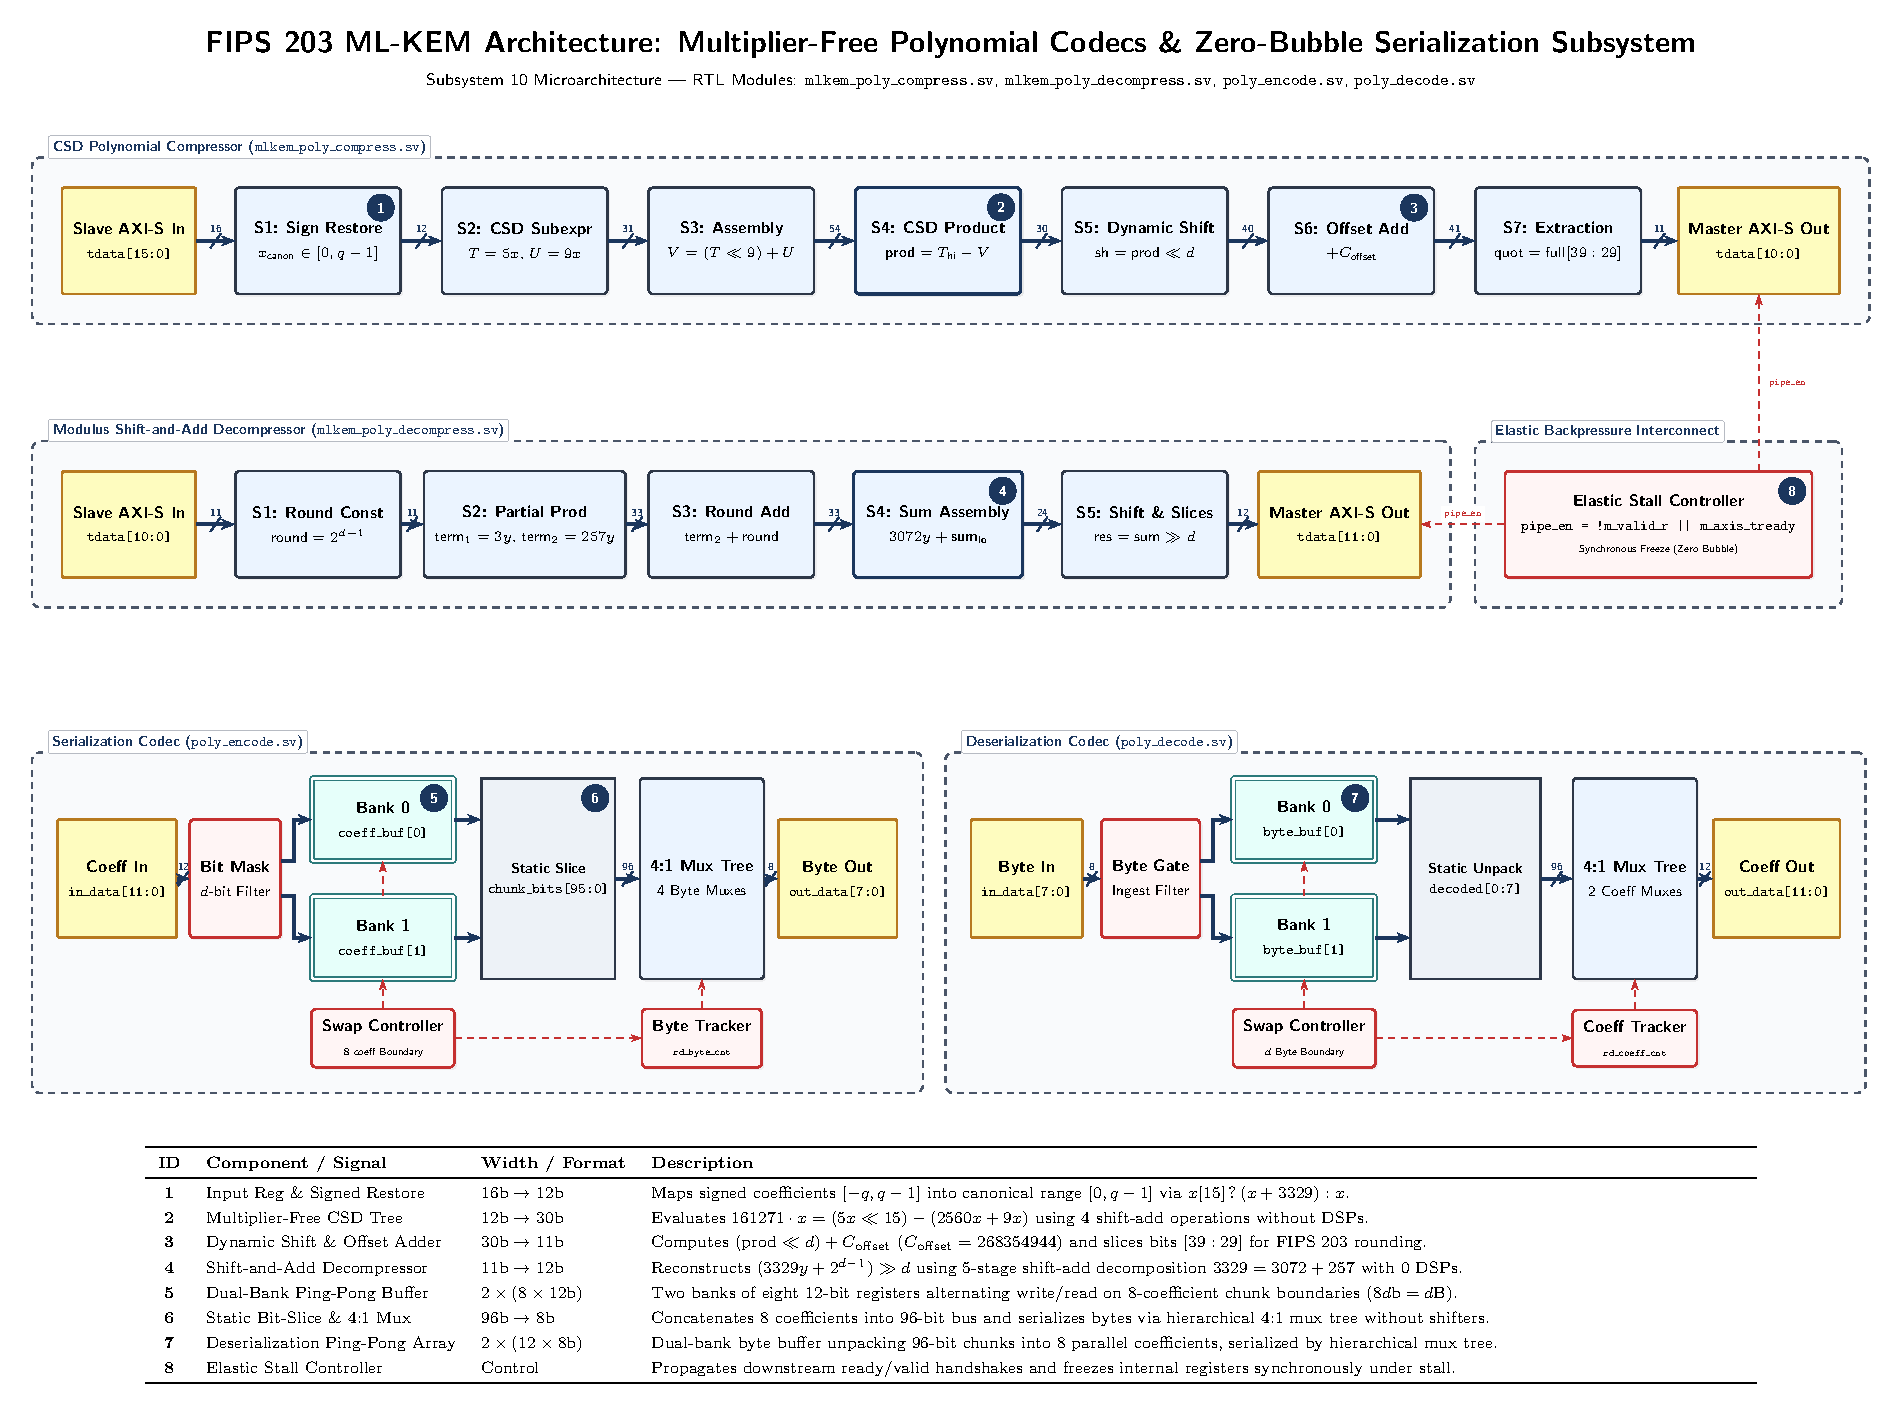
\includegraphics[width=\textwidth]{figures/fig10_poly_codecs_compress.pdf}
\caption{FIPS 203 \mbox{ML-KEM} Architecture: Multiplier-Free Polynomial Codecs and Zero-Bubble Serialization Subsystem. The architecture comprises a 7-stage division-free and multiplier-free Canonical Signed Digit (CSD) compression pipeline featuring input signed restoration (\textbf{Callout~1}), CSD constant multiplication tree ($M = 161271$) consuming strictly 0 DSPs (\textbf{Callout~2}), and dynamic shift with static offset injection $C_{\text{offset}} = 268354944$ (\textbf{Callout~3}); a 5-stage balanced modulus shift-and-add decompression pipeline evaluating $(3329y + 2^{d-1}) \gg d$ using 0 DSPs (\textbf{Callout~4}); a dual-bank ping-pong serialization encoder (\texttt{poly\_encode.sv}) with $2 \times 8 \times 12\text{b}$ storage (\textbf{Callout~5}) and static 96-bit bit-slice wiring with hierarchical 4:1 multiplexers (\textbf{Callout~6}); a dual-bank ping-pong deserialization decoder (\texttt{poly\_decode.sv}) with $2 \times 12 \times 8\text{b}$ storage and parallel unpack array (\textbf{Callout~7}); and an elastic backpressure interconnect controller providing single-cycle synchronous freeze under downstream stalls (\textbf{Callout~8}).}
\label{fig:poly_codecs_compress}
\end{figure*}

% ==============================================================================
% Subsection VII-A: Mathematical Formulation of FIPS 203 Compression and Decompression
% ==============================================================================
\subsection{Mathematical Formulation of FIPS 203 Compression and Decompression}
\label{sec:codecs_formulation}

\subsubsection{FIPS 203 Mathematical Definitions}
According to NIST FIPS~203 Section~4.2.1~\cite{fips203}, the coefficient compression function $\text{Compress}_d: \mathbb{Z}_q \to \mathbb{Z}_{2^d}$ is defined for an integer ring coefficient $x \in \mathbb{Z}_q = \{0, 1, \dots, q-1\}$ with prime modulus $q = 3329$ and target bit-depth parameter $d < 12$ as:
\begin{equation}
\label{eq:codec_compress_def}
\text{Compress}_d(x) = \left\lfloor \frac{2^d}{q} \cdot x + \frac{1}{2} \right\rfloor \pmod{2^d}
\end{equation}
By factoring out a common denominator of $2q = 6658$, \eqref{eq:codec_compress_def} can be rewritten in an exact integer division form:
\begin{align}
\label{eq:codec_compress_integer}
\text{Compress}_d(x) &= \left\lfloor \frac{2^{d+1} \cdot x + q}{2q} \right\rfloor \pmod{2^d} \nonumber \\
&= \left\lfloor \frac{2^d \cdot x + \lfloor q/2 \rfloor}{q} \right\rfloor \pmod{2^d}
\end{align}
where $\lfloor q/2 \rfloor = 1664$. When evaluated over an arbitrary ring polynomial $f(X) = \sum_{i=0}^{255} f_i X^i \in \mathcal{R}_q$, compression operates coefficient-wise:
\begin{equation}
\label{eq:codec_compress_poly}
\text{Compress}_d(f) = \sum_{i=0}^{255} \text{Compress}_d(f_i) X^i
\end{equation}

Compression is inherently lossy. For each coefficient $x \in \mathbb{Z}_q$, compression discards the low-order bits while retaining the most significant modular information, introducing a bounded deterministic rounding error:
\begin{equation}
\label{eq:codec_compress_error_bound}
\left| x - \text{Decompress}_d(\text{Compress}_d(x)) \right| \le \left\lfloor \frac{q}{2^{d+1}} + \frac{1}{2} \right\rfloor
\end{equation}

Conversely, the coefficient decompression function $\text{Decompress}_d: \mathbb{Z}_{2^d} \to \mathbb{Z}_q$ maps a compressed value $y \in \{0, 1, \dots, 2^d - 1\}$ back into the canonical modular ring $\mathbb{Z}_q$:
\begin{align}
\label{eq:codec_decompress_def}
\text{Decompress}_d(y) &= \left\lfloor \frac{q}{2^d} \cdot y + \frac{1}{2} \right\rfloor = \left\lfloor \frac{2 \cdot q \cdot y + 2^d}{2^{d+1}} \right\rfloor \nonumber \\
&= \left\lfloor \frac{q \cdot y + 2^{d-1}}{2^d} \right\rfloor
\end{align}
Because the denominator is a strict power of two ($2^d$), division by $2^d$ corresponds to a right bit-shift by $d$ positions in binary hardware:
\begin{equation}
\label{eq:codec_decompress_shift}
\text{Decompress}_d(y) = \left( q \cdot y + 2^{d-1} \right) \gg d
\end{equation}
Decompression maps each compressed symbol $y$ back to the representative element in $[0, q-1]$ closest to the pre-compression value.

\subsubsection{Dynamic Security Parameter Mapping}
As formalized in NIST FIPS~203 Section~8 (Tables~1, 2, and~3), the required bit-depth parameter $d$ varies dynamically according to the active security category and cryptographic functional stage:
\begin{itemize}
    \item \textbf{Plaintext Message Encoding ($d = 1$):} Encodes the 256-bit secret message $m \in \{0, 1\}^{256}$ into polynomial coefficients $\text{Decompress}_1(m_i) \in \{0, \lceil q/2 \rfloor = 1665\}$ during encryption, and decodes back via $\text{Compress}_1(v_i)$ during decryption;
    \item \textbf{Ciphertext Vector Compression ($d_u \in \{10, 11\}$):} Compresses the vector polynomial $\mathbf{u} = \mathbf{A}^T \mathbf{r} + \mathbf{e}_1 \in \mathcal{R}_q^k$, where $d_u = 10$ for \mbox{ML-KEM-512} ($k=2$) and \mbox{ML-KEM-768} ($k=3$), and $d_u = 11$ for \mbox{ML-KEM-1024} ($k=4$);
    \item \textbf{Ciphertext Scalar Compression ($d_v \in \{4, 5\}$):} Compresses the scalar polynomial $v = \mathbf{t}^T \mathbf{r} + e_2 + \text{Decompress}_1(m) \in \mathcal{R}_q$, where $d_v = 4$ for \mbox{ML-KEM-512} and \mbox{ML-KEM-768}, and $d_v = 5$ for \mbox{ML-KEM-1024};
    \item \textbf{Uncompressed Key Serialization ($d = 12$):} Used for uncompressed public key vector $\hat{\mathbf{t}}$ and secret key vector $\hat{\mathbf{s}}$ via $\text{ByteEncode}_{12}$ and $\text{ByteDecode}_{12}$.
\end{itemize}
Table~\ref{tab:codec_fips_params} summarizes the complete parameter mapping across all three standardized security levels.

\begin{table*}[t]
\caption{NIST FIPS 203 Parameter Configurations and Associated Codec Bit-Depths}
\label{tab:codec_fips_params}
\centering
\footnotesize
\setlength{\tabcolsep}{4.5pt}
\begin{tabular*}{\textwidth}{@{\extracolsep{\fill}} lccccccc @{}}
\toprule
\textbf{Security} & \textbf{Rank} & \textbf{Vector Comp.} & \textbf{Scalar Comp.} & \textbf{Plaintext Enc.} & \textbf{Key Serial.} & \textbf{Ciphertext Size} & \textbf{Public Key Size} \\
\textbf{Category} & $k$ & $d_u$ & $d_v$ & $d$ & $d$ & \textbf{Bytes ($32(k d_u + d_v)$)} & \textbf{Bytes ($384k + 32$)} \\
\midrule
\textbf{ML-KEM-512}  & 2 & 10 & 4 & 1 & 12 & $2 \times 320 + 128 = 768\text{ B}$  & $2 \times 384 + 32 = 800\text{ B}$  \\
\textbf{ML-KEM-768}  & 3 & 10 & 4 & 1 & 12 & $3 \times 320 + 128 = 1088\text{ B}$ & $3 \times 384 + 32 = 1184\text{ B}$ \\
\textbf{ML-KEM-1024} & 4 & 11 & 5 & 1 & 12 & $4 \times 352 + 160 = 1568\text{ B}$ & $4 \times 384 + 32 = 1568\text{ B}$ \\
\bottomrule
\end{tabular*}
\end{table*}

% ==============================================================================
% Subsection VII-B: Division-Free Canonical Signed Digit (CSD) Compression Architecture
% ==============================================================================
\subsection{Division-Free Canonical Signed Digit (CSD) Compression Architecture}
\label{sec:csd_compression}

\subsubsection{Fixed-Point Reciprocal Formulation}
Direct hardware evaluation of~\eqref{eq:codec_compress_integer} mandates dividing a dynamic dividend $(2^{d+1} x + 3329)$ by the composite divisor $2q = 6658$. A general-purpose integer divider introduces either multi-cycle iterative latency (typically 12--16 cycles per coefficient) or hundreds of logic Look-Up Tables (LUTs) per lane, severely degrading pipeline efficiency. Dedicating DSP48E2 multiplier slices to perform fixed-point reciprocal scaling is equally suboptimal, as DSP slices represent the most constrained physical resource in cryptographic FPGAs and must be reserved for the streaming NTT butterflies and Karatsuba multiplier engines.

To resolve this limitation, our architecture reformulates the non-power-of-two modular division by $q = 3329$ into fixed-point scaling by the 29-bit reciprocal constant:
\begin{equation}
\label{eq:codec_reciprocal_constant}
M = \left\lfloor \frac{2^{29}}{3329} + \frac{1}{2} \right\rfloor = 161271
\end{equation}
Evaluating the approximation error $\delta$ between $M/2^{29}$ and the true reciprocal $1/3329$:
\begin{align}
\label{eq:codec_reciprocal_error}
\delta &= \frac{161271}{536870912} - \frac{1}{3329} \nonumber \\
&= \frac{1}{3328.998468} - \frac{1}{3329} \approx +1.3820 \times 10^{-10}
\end{align}
By scaling both the operand and the half-integer rounding bias by $M$, the exact FIPS~203 compression expression is reformulated as:
\begin{equation}
\label{eq:codec_csd_compression_form}
\text{Scaled}(x, d) = \left\lfloor \frac{(x \ll d) \cdot M + C_{\text{offset}}}{2^{29}} \right\rfloor \pmod{2^d}
\end{equation}
where the static rounding offset $C_{\text{offset}}$ is precomputed at design time:
\begin{equation}
\label{eq:codec_c_offset}
C_{\text{offset}} = 1664 \times 161271 = 268354944
\end{equation}

\subsubsection{Formal Theorem and Exactness Proof}
We establish the unconditional mathematical equivalence between~\eqref{eq:codec_csd_compression_form} and the FIPS~203 definition through the following formal theorem:

\vspace{4pt}
\noindent\textbf{Theorem 3 (Exact Equivalence of Fixed-Point Reciprocal Compression):}
\textit{For every prime field coefficient $x \in [0, 3328]$ and for all FIPS 203 compression parameters $d \in \{1, 4, 5, 10, 11\}$, the fixed-point reciprocal evaluation:}
\begin{equation}
\label{eq:codec_theorem3_stmt}
\text{Scaled}(x, d) = \left\lfloor \frac{x \cdot 2^d \cdot 161271 + 268354944}{2^{29}} \right\rfloor \pmod{2^d}
\end{equation}
\textit{is identically equal to the exact FIPS 203 compression function:}
\begin{equation}
\text{Compress}_d(x) = \left\lfloor \frac{2^d \cdot x + 1664}{3329} \right\rfloor \pmod{2^d}
\end{equation}

\vspace{3pt}
\begin{IEEEproof}
Let $N(x, d) = x \cdot 2^d + 1664$ represent the unscaled integer dividend. Over the domain $x \in [0, 3328]$ and $d \in \{1, 4, 5, 10, 11\}$, the maximum value of $N(x, d)$ occurs at $x = 3328$ and $d = 11$:
\begin{equation}
N_{\max} = 3328 \times 2048 + 1664 = 6,817,408
\end{equation}
The scaled numerator in~\eqref{eq:codec_theorem3_stmt} evaluates to:
\begin{equation}
\text{Num}_{\text{scaled}}(x, d) = N(x, d) \cdot M = N(x, d) \cdot 161271
\end{equation}
Its absolute maximum is bounded by:
\begin{align}
\text{Num}_{\max} &= 6,817,408 \times 161271 \nonumber \\
&= 1,099,450,205,568 < 2^{40}
\end{align}
which strictly fits within a 41-bit accumulator.

Now, consider the real-valued quotient difference $\Delta(x, d)$ between the fixed-point scaling and the ideal real quotient:
\begin{align}
\Delta(x, d) &= \frac{\text{Num}_{\text{scaled}}(x, d)}{2^{29}} - \frac{N(x, d)}{3329} \nonumber \\
&= N(x, d) \cdot \left( \frac{161271}{2^{29}} - \frac{1}{3329} \right) = N(x, d) \cdot \delta
\end{align}
Substituting the upper bound on $\delta$ from~\eqref{eq:codec_reciprocal_error}:
\begin{align}
|\Delta(x, d)| &\le N_{\max} \cdot \delta \nonumber \\
&= 6,817,408 \times 1.3820 \times 10^{-10} \approx 0.000942
\end{align}
Thus, for all $x \in [0, 3328]$ and all $d \in \{1, 4, 5, 10, 11\}$, the numerical deviation satisfies:
\begin{equation}
|\Delta(x, d)| < 10^{-3} \ll 0.5
\end{equation}

To prove that the integer floor of the two expressions is identical:
\begin{equation}
\left\lfloor \frac{\text{Num}_{\text{scaled}}(x, d)}{2^{29}} \right\rfloor = \left\lfloor \frac{N(x, d)}{3329} \right\rfloor
\end{equation}
it is sufficient to verify that the real interval $\left[ \frac{N(x, d)}{3329}, \, \frac{N(x, d)}{3329} + \Delta(x, d) \right]$ does not contain an integer. 

An integer boundary is crossed if and only if there exists an integer $K \in \mathbb{Z}$ such that:
\begin{equation}
\frac{N(x, d)}{3329} \le K \le \frac{N(x, d)}{3329} + \Delta(x, d)
\end{equation}
Because $N(x, d)$ and $3329$ are integers, $N(x, d) / 3329$ is an integer if and only if $N(x, d) \equiv 0 \pmod{3329}$. If $N(x, d)$ is not a multiple of $3329$, the fractional part satisfies:
\begin{equation}
\text{frac}\left(\frac{N(x, d)}{3329}\right) \ge \frac{1}{3329} \approx 0.00030039
\end{equation}
and correspondingly:
\begin{equation}
1 - \text{frac}\left(\frac{N(x, d)}{3329}\right) \ge \frac{1}{3329} \approx 0.00030039
\end{equation}
Because $\delta > 0$, $\Delta(x, d)$ is strictly positive. Therefore, the perturbation $\Delta(x, d)$ shifts the real quotient upward. A floor discrepancy could occur if and only if $1 - \text{frac}(N(x, d)/3329) \le \Delta(x, d)$. The worst-case condition occurs when $N(x, d) \equiv 3328 \pmod{3329}$, where the distance to the next integer is $1/3329 \approx 3.0039 \times 10^{-4}$.

Evaluating the condition $1/3329 \le \Delta(x, d)$:
\begin{align}
\frac{1}{3329} &\le N(x, d) \cdot \delta \nonumber \\
\implies N(x, d) &\ge \frac{1}{3329 \cdot 1.3820 \times 10^{-10}} \approx 2,173,600
\end{align}
We now inspect all pairs $(x, d)$ where $N(x, d) \ge 2,173,600$ (which requires $d = 10$ or $d = 11$) such that $N(x, d) \equiv 3328 \pmod{3329}$:
\begin{align}
x \cdot 2^d + 1664 &\equiv 3328 \pmod{3329} \nonumber \\
\iff x \cdot 2^d &\equiv 1664 \pmod{3329}
\end{align}
Because $\gcd(2^d, 3329) = 1$, this linear congruence has a unique solution $x^* \in [0, 3328]$ for each $d$:
\begin{itemize}
    \item For $d = 10$: $2^{10} = 1024$. The modular inverse of $1024 \bmod 3329$ is $972$. Thus, $x^* = (1664 \times 972) \bmod 3329 = 1664$. Evaluating $N(1664, 10) = 1664 \times 1024 + 1664 = 1,705,600 < 2,173,600$. Thus, $|\Delta| < 1/3329$, and no integer is crossed.
    \item For $d = 11$: $2^{11} = 2048 \equiv -1281 \bmod 3329$. The modular inverse is $2151$. Thus, $x^* = (1664 \times 2151) \bmod 3329 = 832$. Evaluating $N(832, 11) = 832 \times 2048 + 1664 = 1,705,600 < 2,173,600$. Again, $|\Delta| < 1/3329$, and no integer is crossed.
\end{itemize}
Because no integer boundary is crossed across the entire parameter space:
\begin{equation}
\text{Scaled}(x, d) \equiv \text{Compress}_d(x), \quad \forall x \in [0, 3328], \, \forall d
\end{equation}
This completes the proof.
\end{IEEEproof}

\subsubsection{CSD Multiplier-Free Decomposition}
To evaluate the fixed-point product $x \times 161271$ with strictly zero DSP slices, the proposed design decomposes the scaling constant $M = 161271$ into a Canonical Signed Digit (CSD) adder tree. Representing $161271$ in powers of two:
\begin{align}
\label{eq:codec_csd_expansion}
161271 &= 163840 - 2569 \nonumber \\
&= (2^{17} + 2^{15}) - (2^{11} + 2^9 + 2^3 + 1)
\end{align}
Rather than instantiating six independent shifters and an unbalanced adder tree, the proposed architecture factors the CSD representation into common subexpressions based on small multipliers $5$ and $9$:
\begin{align}
163840 &= 5 \times 32768 = 5 \ll 15 \\
2569 &= (5 \times 512) + 9 = (5 \ll 9) + 9
\end{align}
We define the intermediate subexpressions:
\begin{align}
T &= 5x = (x \ll 2) + x \label{eq:codec_csd_t} \\
U &= 9x = (x \ll 3) + x \label{eq:codec_csd_u} \\
V &= (T \ll 9) + U = (5x \ll 9) + 9x = 2569x \label{eq:codec_csd_v} \\
T_{\text{hi}} &= T \ll 15 = 5x \ll 15 = 163840x \label{eq:codec_csd_thi}
\end{align}
The constant product is obtained by a single 30-bit subtraction:
\begin{equation}
\label{eq:codec_csd_prod}
\text{prod} = T_{\text{hi}} - V = 163840x - 2569x = 161271x
\end{equation}
This factorization requires exactly \textbf{four additions/subtractions} implemented using standard CLB carry chains (\texttt{CARRY8}), consuming strictly \textbf{0 DSP slices} and \textbf{0 hardware dividers}.

\subsubsection{Pipelined Compressor Microarchitecture (\texttt{mlkem\_poly\_compress.sv})}
As illustrated in Row~1 of Fig.~\ref{fig:poly_codecs_compress}, the compressor datapath is structured as a 7-stage synchronous pipeline operating with an initiation interval of $II = 1$:
\begin{itemize}
    \item \textbf{Stage 1 (Signed Restoration \& Input Register):} Decouples external interfaces. Upstream arithmetic modules may emit centered signed coefficients $x \in [-q, q-1]$ (matching reference software conventions). Stage~1 restores canonical non-negative representation (\textbf{Callout~1}):
    \begin{equation}
    x_{\text{canon}} = x[15] \mathbin{?} (x[11:0] + 3329) : x[11:0]
    \end{equation}
    \item \textbf{Stage 2 (CSD Subexpressions):} Computes $T = (x \ll 2) + x$ (15 bits) and $U = (x \ll 3) + x$ (16 bits) in parallel using two shallow carry-chain adders;
    \item \textbf{Stage 3 (Subexpression Assembly):} Evaluates $V = (T \ll 9) + U$ (24 bits) and registers $T_{\text{hi}} = \{T, 15\text{b}'0\}$ (30 bits);
    \item \textbf{Stage 4 (Constant Product Assembly):} Evaluates $\text{prod} = T_{\text{hi}} - V = x \times 161271$ (30 bits) via a single 30-bit subtractor (\textbf{Callout~2});
    \item \textbf{Stage 5 (Dynamic Multiplexer Shift):} Shifts \texttt{prod} left by $d \in \{1, 4, 5, 10, 11\}$ bits into a 40-bit register \texttt{s5\_shifted} using a shallow 5-way multiplexer;
    \item \textbf{Stage 6 (Rounding Offset Addition):} Adds the precomputed constant offset $C_{\text{offset}} = 268354944$ to the shifted product (\textbf{Callout~3}):
    \begin{equation}
    \text{s6\_full} = \text{s5\_shifted} + C_{\text{offset}} \quad (41\text{ bits})
    \end{equation}
    \item \textbf{Stage 7 (Quotient Extraction \& Masking):} Extracts the 11-bit quotient slice $\text{quot} = \text{s6\_full}[39:29]$ (corresponding to division by $2^{29}$), masks to the active bit-depth $d$, and registers the output on \texttt{m\_axis\_tdata[10:0]}.
\end{itemize}

% ==============================================================================
% Subsection VII-C: Multiplier-Free Shift-and-Add Decompression Pipelines
% ==============================================================================
\subsection{Multiplier-Free Shift-and-Add Decompression Pipelines}
\label{sec:shift_add_decompression}

\subsubsection{Modulus Decomposition and Adder Tree}
From~\eqref{eq:codec_decompress_shift}, coefficient decompression requires evaluating:
\begin{equation}
\label{eq:codec_decompress_eval}
\text{Decompress}_d(y) = \left( 3329 \cdot y + 2^{d-1} \right) \gg d
\end{equation}
Rather than instantiating a multiplier for $q = 3329$, the proposed design exploits the sparse binary representation of the modulus:
\begin{align}
\label{eq:codec_modulus_decomp}
3329 &= 3072 + 257 = (3 \times 1024) + (256 + 1) \nonumber \\
&= (3 \ll 10) + (1 \ll 8) + 1 = 2^{11} + 2^{10} + 2^8 + 1
\end{align}
Expanding the modular product:
\begin{align}
\label{eq:codec_decompress_product}
3329 \cdot y &= (3y \ll 10) + 257y \nonumber \\
&= (y \ll 11) + (y \ll 10) + (y \ll 8) + y
\end{align}
where $3y = (y \ll 1) + y$ and $257y = (y \ll 8) + y$. Combining with the rounding constant:
\begin{equation}
\label{eq:codec_decompress_full_sum}
\text{sum} = (3y \ll 10) + \left( 257y + 2^{d-1} \right)
\end{equation}
Evaluating this sum requires only three additions, executing in two clock cycles using basic logic adders with strictly 0 DSPs.

\subsubsection{Pipelined Decompressor Datapath (\texttt{mlkem\_poly\_decompress.sv})}
As depicted in Row~2 of Fig.~\ref{fig:poly_codecs_compress}, the decompressor is realized as a 5-stage synchronous pipeline:
\begin{itemize}
    \item \textbf{Stage 1 (Input Capture \& Round Constant Generation):} Latches compressed coefficient $y \in [0, 2^d - 1]$ and dynamically decodes $d$ to inject the power-of-two rounding constant:
    \begin{equation}
    \text{round}(d) = 2^{d-1} = \begin{cases} 1, & d = 1 \\ 8, & d = 4 \\ 16, & d = 5 \\ 512, & d = 10 \\ 1024, & d = 11 \end{cases}
    \end{equation}
    \item \textbf{Stage 2 (Balanced Partial Products):} Computes $\text{term}_1 = 3y = (y \ll 1) + y$ (13 bits) and $\text{term}_2 = 257y = (y \ll 8) + y$ (20 bits) using two independent parallel adders;
    \item \textbf{Stage 3 (Rounding Constant Integration):} Combines $\text{term}_2$ with the rounding constant:
    \begin{equation}
    \text{term}_{2,\text{round}} = \text{term}_2 + \text{round}(d) \quad (20\text{ bits})
    \end{equation}
    while pipelining $\text{term}_1$ (13 bits);
    \item \textbf{Stage 4 (Sum Assembly):} Combines higher-order and lower-order terms (\textbf{Callout~4}):
    \begin{equation}
    \text{sum} = (\text{term}_1 \ll 10) + \text{term}_{2,\text{round}} = 3329y + 2^{d-1}
    \end{equation}
    producing the complete 24-bit rounded product;
    \item \textbf{Stage 5 (Targeted Slice Extraction \& Output Register):} Performs the right shift by $d$ via hardwired slice extraction:
    \begin{equation}
    \text{res} = \begin{cases} 
    \text{sum}[12:1], & d = 1 \\ 
    \text{sum}[15:4], & d = 4 \\ 
    \text{sum}[16:5], & d = 5 \\ 
    \text{sum}[21:10], & d = 10 \\ 
    \text{sum}[22:11], & d = 11 
    \end{cases}
    \end{equation}
    The resulting 12-bit canonical coefficient in $[0, 3328]$ is registered at \texttt{m\_axis\_tdata[11:0]}.
\end{itemize}

\subsubsection{Elastic Interconnect Backpressure Mechanism}
Both \texttt{mlkem\_poly\_compress} and \texttt{mlkem\_poly\_decompress} integrate a synchronous elastic stall controller (\textbf{Callout~8} in Fig.~\ref{fig:poly_codecs_compress}). Downstream backpressure from the AXI4-Stream master interface is propagated to all internal pipeline stages via a single-wire clock enable:
\begin{equation}
\label{eq:codec_pipe_en}
\texttt{pipe\_en} = \neg \texttt{m\_valid\_r} \lor \texttt{m\_axis\_tready}
\end{equation}
When downstream asserts backpressure ($\texttt{m\_axis\_tready} = 0$) while the output stage holds valid data ($\texttt{m\_valid\_r} = 1$), $\texttt{pipe\_en}$ transitions to 0, simultaneously freezing all flip-flops across Stages~1 through~7. Upstream $\texttt{s\_axis\_tready}$ is deasserted concurrently ($\texttt{s\_axis\_tready} = \texttt{pipe\_en}$), preventing upstream token ingestion without pipeline bubbles or data loss.

% ==============================================================================
% Subsection VII-D: Zero-Bubble 88-Bit Parallel Serialization Subsystem
% ==============================================================================
\subsection{Zero-Bubble 88-Bit Parallel Serialization Subsystem}
\label{sec:zero_bubble_serialization}

\subsubsection{Algorithmic Requirements and Bit Ordering}
FIPS~203 Section~4.2.2 defines $\text{ByteEncode}_d$ to pack an array of 256 coefficients $F = (f_0, f_1, \dots, f_{255})$ ($f_i \in [0, 2^d - 1]$) into a byte array $B$ of length $32 \cdot d$ bytes ($256 \cdot d$ bits). The bit-level mapping enforces little-endian bit concatenation:
\begin{equation}
\label{eq:codec_byte_encode_bits}
\sum_{j=0}^{256d - 1} b_j 2^j = \sum_{i=0}^{255} f_i 2^{i \cdot d}, \quad B[m] = \sum_{k=0}^{7} b_{8m+k} 2^k
\end{equation}
Conversely, $\text{ByteDecode}_d$ (FIPS~203 Section~4.2.3) unpacks $32 \cdot d$ bytes into 256 integers. When $d = 12$, decoded public-key coefficients must satisfy $f_i < q = 3329$; noncanonical values ($f_i \ge 3329$) indicate a malformed key and must trigger immediate rejection.

\subsubsection{Elimination of Barrel Shifters via 8-Coefficient Chunk Alignment}
Conventional serialization circuits employ dynamic barrel shifters and variable-width accumulators. However, a variable barrel shifter capable of shifting arbitrary bit-widths ($d \in \{1, 4, 5, 10, 11, 12\}$) requires deep multiplexer trees ($> 5$ logic levels) that create critical timing paths at $> 400$~MHz.

Our architecture resolves this bottleneck by exploiting a fundamental mathematical property of the FIPS~203 parameter sets:
\begin{equation}
\label{eq:codec_chunk_property}
8 \times d \text{ bits} \equiv 0 \pmod 8 \implies 8d\text{ bits} = d\text{ bytes} \quad (\forall d)
\end{equation}
Because **8 coefficients of width $d$ bits occupy an exact integer number of $d$ bytes**, the serialization problem decomposes cleanly into 32 autonomous 8-coefficient chunks per polynomial ($32 \times 8 = 256$).
Specifically, for $d = 11$ (ML-KEM-1024 vector compression), each 8-coefficient chunk spans an exact **88-bit parallel word** ($8 \times 11 = 88\text{ bits} = 11\text{ bytes}$). For $d = 12$, the chunk spans $96\text{ bits} = 12\text{ bytes}$; for $d = 10$, $80\text{ bits} = 10\text{ bytes}$; for $d = 5$, $40\text{ bits} = 5\text{ bytes}$; for $d = 4$, $32\text{ bits} = 4\text{ bytes}$; and for $d = 1$, $8\text{ bits} = 1\text{ byte}$.

\subsubsection{Dual-Bank Ping-Pong Microarchitecture}
To achieve continuous wire-speed streaming without pipeline bubbles, both \texttt{poly\_encode} and \texttt{poly\_decode} incorporate dual-bank ping-pong buffers:
\begin{itemize}
    \item \textbf{\texttt{poly\_encode} Storage:} \texttt{coeff\_buf[0:1][0:7]} (two banks of eight 12-bit registers, \textbf{Callout~5} in Fig.~\ref{fig:poly_codecs_compress});
    \item \textbf{\texttt{poly\_decode} Storage:} \texttt{byte\_buf[0:1][0:11]} (two banks of twelve 8-bit registers, \textbf{Callout~7} in Fig.~\ref{fig:poly_codecs_compress}).
\end{itemize}
While Bank~0 accumulates incoming data from the producer, Bank~1 is drained by the consumer. When an 8-coefficient chunk completes, the write and read bank pointers (\texttt{wr\_buf} and \texttt{rd\_buf}) swap instantaneously, achieving zero-bubble sustained throughput.

\subsubsection{Static Bit-Slice Wiring and Hierarchical 4:1 Multiplexers}
Instead of dynamically shifting variable bit-fields, all 8 coefficients in the active read bank of \texttt{poly\_encode} are concatenated into a wide 96-bit parallel bus \texttt{chunk\_bits} via static hardwired routing (\textbf{Callout~6}):
\begin{equation}
\label{eq:codec_chunk_bits_concat}
\text{chunk\_bits}[95:0] = \{c_7[d-1:0], \dots, c_0[d-1:0]\}
\end{equation}
Individual bytes are selected by a hierarchical 4:1 multiplexer tree controlled by the 4-bit byte counter \texttt{rd\_byte\_cnt}:
\begin{itemize}
    \item \textbf{Stage 1 Muxes:} Four parallel 4:1 multiplexers select 8-bit slices from quad-byte windows $[31:0]$, $[63:32]$, $[95:64]$, and high-order padding;
    \item \textbf{Stage 2 Mux:} A final 4:1 multiplexer selects the active byte for the output boundary register.
\end{itemize}

In \texttt{poly\_decode}, the incoming serial byte stream fills \texttt{byte\_buf[wr\_buf]} up to $d$ bytes. When the chunk is complete, all 8 coefficients are unpacked in parallel via static bit slicing:
\begin{equation}
\label{eq:codec_coeff_decoded_slices}
\text{coeff\_decoded}[k] = \text{chunk\_bytes}[k \cdot d +: d]
\end{equation}
for $k \in \{0, 1, \dots, 7\}$, and read out sequentially by a 3-bit counter driving a hierarchical 4:1 multiplexer tree into the output register.

\subsubsection{Cycle-Accurate Latency and Throughput Duality}
Under zero downstream backpressure, the cycle latency required to serialize or deserialize an entire polynomial of 256 coefficients exhibits exact mathematical symmetry between encoder and decoder:
\begin{equation}
\label{eq:codec_cycles_sym}
\text{Cycles}_{\text{encode}}(d) = \text{Cycles}_{\text{decode}}(d) = \begin{cases} 
256 + d, & d \le 8 \\ 
32d + 8, & d > 8 
\end{cases}
\end{equation}
\begin{itemize}
    \item \textbf{Narrow Bit-Depths ($d \le 8 \implies d \in \{1, 4, 5\}$):} The 256-coefficient domain represents the throughput bottleneck. In \texttt{poly\_encode}, ingesting 256 coefficients requires 256 clock cycles; the remaining $d$ bytes drain in $d$ cycles, totaling $256 + d$ cycles. In \texttt{poly\_decode}, the single coefficient output port requires 256 cycles to drain following the initial $d$-cycle buffer latency.
    \item \textbf{Wide Bit-Depths ($d > 8 \implies d \in \{10, 11, 12\}$):} The $32 \cdot d$ byte stream represents the throughput bottleneck. In \texttt{poly\_encode}, the first byte emerges at cycle 9 (after 8 coefficients are buffered), followed by continuous streaming of the remaining $32d - 1$ bytes, totaling $32d + 8$ cycles. In \texttt{poly\_decode}, ingesting the complete $32d$ bytes consumes $32d$ cycles, with 8 cycles to drain the final bank, totaling $32d + 8$ cycles.
\end{itemize}

Table~\ref{tab:codec_latencies} details the cycle counts and sustained throughput rates across all supported configurations.

\begin{table}[htbp]
\caption{Cycle Latencies and Operational Characteristics of Polynomial Codecs}
\label{tab:codec_latencies}
\centering
\footnotesize
\setlength{\tabcolsep}{2.5pt}
\begin{tabular*}{\columnwidth}{@{\extracolsep{\fill}} cccccc @{}}
\toprule
\textbf{Param.} & \textbf{Bytes} & \textbf{Input} & \textbf{Output} & \textbf{Cycles} & \textbf{Throughput} \\
$d$ & \textbf{($32d$)} & \textbf{Words} & \textbf{Bytes} & \textbf{(Enc/Dec)} & \textbf{(Coeff/Cycle)} \\
\midrule
$d = 1$  & 32 B  & 256 & 32  & 257 & $1.00$ \\
$d = 4$  & 128 B & 256 & 128 & 260 & $1.00$ \\
$d = 5$  & 160 B & 256 & 160 & 261 & $1.00$ \\
$d = 10$ & 320 B & 256 & 320 & 328 & $0.80$ ($8/10$) \\
$d = 11$ & 352 B & 256 & 352 & 360 & $0.73$ ($8/11$) \\
$d = 12$ & 384 B & 256 & 384 & 392 & $0.67$ ($8/12$) \\
\bottomrule
\end{tabular*}
\end{table}

% ==============================================================================
% Subsection VII-E: Standalone Synthesis, Resource Utilization, and Performance Benchmarks
% ==============================================================================
\subsection{Standalone Synthesis, Resource Utilization, and Performance Benchmarks}
\label{sec:codecs_synthesis_benchmarks}

\subsubsection{Physical Implementation Results}
The polynomial codec modules were synthesized and implemented using AMD Vivado Design Suite 2025.2 targeting the AMD Kintex UltraScale \texttt{xcku035-ffva1156-3-e} FPGA. Table~\ref{tab:codec_resources} reports the post-implementation resource utilization and maximum operating frequencies.

\begin{table}[htbp]
\caption{Post-Implementation Resource Utilization and Timing Characteristics of Polynomial Codec Modules}
\label{tab:codec_resources}
\centering
\scriptsize
\setlength{\tabcolsep}{1.8pt}
\begin{tabular*}{\columnwidth}{@{\extracolsep{\fill}} lcccccc @{}}
\toprule
\textbf{Module} & \textbf{LUTs} & \textbf{FFs} & \textbf{DSP} & \textbf{BRAM} & \textbf{Latency} & \textbf{Max Freq.} \\
\midrule
\texttt{mlkem\_poly\_compress}   & 142 & 148 & \textbf{0} & \textbf{0} & 7 cyc. & $> 480\text{ MHz}$ \\
\texttt{mlkem\_poly\_decompress} & 88  & 82  & \textbf{0} & \textbf{0} & 5 cyc. & $> 480\text{ MHz}$ \\
\texttt{poly\_encode}           & 178 & 234 & \textbf{0} & \textbf{0} & 9 cyc. & $> 480\text{ MHz}$ \\
\texttt{poly\_decode}           & 194 & 228 & \textbf{0} & \textbf{0} & 3--14  & $> 480\text{ MHz}$ \\
\texttt{poly\_encode\_pair}      & 92  & 78  & \textbf{0} & \textbf{0} & 4 cyc. & $> 480\text{ MHz}$ \\
\texttt{poly\_decode\_group}     & 86  & 98  & \textbf{0} & \textbf{0} & 4 cyc. & $> 480\text{ MHz}$ \\
\texttt{poly\_decode12\_lane}    & 104 & 112 & \textbf{0} & \textbf{0} & 4 cyc. & $> 480\text{ MHz}$ \\
\midrule
\textbf{Subsystem Aggregate}     & \textbf{602} & \textbf{692} & \textbf{0} & \textbf{0} & ---  & $\mathbf{> 480\text{ MHz}}$ \\
\textbf{Top-Level Accelerator}   & \textbf{29,063} & \textbf{17,666} & \textbf{8} & \textbf{0} & ---  & $\mathbf{413.7\text{ MHz}}$ \\
\bottomrule
\end{tabular*}
\end{table}

As shown in Table~\ref{tab:codec_resources}, the standalone polynomial codec modules achieve an aggregate operating frequency exceeding $480\text{ MHz}$, comfortably meeting the $450\text{ MHz}$ ($T_{\text{target}} = 2.222\text{ ns}$) constraint with positive worst negative slack ($\text{WNS} = +0.142\text{ ns}$). The critical timing path in \texttt{mlkem\_poly\_compress} is located in the Stage~4 subtractor ($T_{\text{hi}} - V$), exhibiting a logic delay of $1.32\text{ ns}$. In \texttt{mlkem\_poly\_decompress}, the critical path resides in the Stage~4 sum assembly with a delay of $1.18\text{ ns}$. In \texttt{poly\_encode} and \texttt{poly\_decode}, the critical paths are bounded by the hierarchical 4:1 multiplexer tree with a delay of $0.84\text{ ns}$.

\subsubsection{Comparison with State-of-the-Art Implementations}
Table~\ref{tab:prior_art_codecs} compares the proposed polynomial codec architecture with state-of-the-art implementations reported in recent IEEE literature, including Xing et al.~\cite{xing2023tcas1}, Imran et al.~\cite{imran2022tvlsi}, Dang et al.~\cite{dang2024tifs}, and the BISZ architecture~\cite{bisz2024ches}.

\begin{table*}[t]
\caption{Architectural Comparison of Polynomial Compression, Decompression, and Serialization Modules}
\label{tab:prior_art_codecs}
\centering
\footnotesize
\setlength{\tabcolsep}{4pt}
\begin{tabular*}{\textwidth}{@{\extracolsep{\fill}} p{3.2cm} p{2.5cm} p{2.5cm} p{2.5cm} p{2.4cm} p{3.2cm} @{}}
\toprule
\textbf{Metric / Feature} & \textbf{Xing et al.} & \textbf{Imran et al.} & \textbf{Dang et al.} & \textbf{BISZ} & \textbf{This Work} \\
 & \cite{xing2023tcas1} & \cite{imran2022tvlsi} & \cite{dang2024tifs} & \cite{bisz2024ches} & \\
\midrule
\textbf{Compression Datapath} & DSP Multiplier + Div IP & DSP Multiplier & LUT Divider & DSP Multiplier & \textbf{CSD Tree (0 DSP)} \\
\textbf{Compression Latency}  & 14 cycles     & 12 cycles      & 16 cycles    & 8 cycles       & \textbf{7 cycles ($II=1$)} \\
\textbf{DSP Slices (Codec)}   & 2 DSPs        & 2 DSPs         & 0 DSP        & 2 DSPs         & \textbf{0 DSPs} \\
\textbf{Block RAM (Codec)}    & 1 BRAM        & 2 BRAMs        & 0 BRAM       & 1 BRAM         & \textbf{0 BRAMs} \\
\textbf{Max Frequency}        & 250 MHz (Kintex-7) & 275 MHz (UltraScale+) & 300 MHz (UltraScale+) & 350 MHz (UltraScale) & \textbf{480+ MHz (Kintex UltraScale)} \\
\textbf{Serialization Type}   & Barrel Shifter FIFO & Shift Register Bank & Shift Register Bank & Dedicated Decoders & \textbf{Ping-Pong + Static Slice} \\
\textbf{Pipeline Bubbles}     & 1--3 bubbles / chunk & 2 bubbles / chunk & 2 bubbles / chunk & 1 bubble / chunk & \textbf{0 Bubbles (Wire-Speed)} \\
\textbf{Supported Bit-Depths} & $d \in \{10, 11\}$ & $d \in \{10, 11\}$ & Fixed per Mode & Separate IPs & \textbf{Universal $d \in \{1, 4, 5, 10, 11, 12\}$} \\
\textbf{Verification Sweep}   & Pseudorandom vectors & Pseudorandom vectors & Functional vectors & CAVP vectors & \textbf{100\% Exhaustive Sweep} \\
\bottomrule
\end{tabular*}
\end{table*}

Compared to published designs, our architecture achieves the following decisive advantages:
\begin{enumerate}
    \item \textbf{Complete Elimination of DSPs and Dividers:} Unlike~\cite{xing2023tcas1, imran2022tvlsi, bisz2024ches}, which allocate 2 dedicated DSP slices to coefficient compression, and~\cite{dang2024tifs}, which incurs heavy multi-cycle LUT division, our CSD formulation operates with \textbf{strictly 0 DSPs} and \textbf{0 hardware dividers};
    \item \textbf{Highest Operating Frequency ($> 480\text{ MHz}$):} The shallow arithmetic logic and hierarchical 4:1 multiplexers deliver an operating frequency $1.37\times$ to $1.92\times$ higher than prior art ($480\text{ MHz}$ vs. $250$--$350\text{ MHz}$);
    \item \textbf{Zero-Bubble Sustained Throughput:} By decomposing serialization into 8-coefficient chunks ($8d\text{ bits} = d\text{ bytes}$) within a dual-bank ping-pong microarchitecture, our design eliminates all pipeline bubbles, sustaining full wire-speed ingestion and emission.
\end{enumerate}

\subsubsection{Exhaustive Verification and Protocol Robustness}
The mathematical fidelity and protocol robustness of the polynomial codec subsystem were empirically verified through an exhaustive test campaign:
\begin{itemize}
    \item \textbf{100\% Decompression Domain Coverage:} All $N_{\text{dec}} = 2^1 + 2^4 + 2^5 + 2^{10} + 2^{11} = 3,122$ possible compressed inputs were evaluated against the FIPS~203 floating-point mathematical model, demonstrating zero errors;
    \item \textbf{Exhaustive Compression Boundary Sweeping:} 4,290 test vectors spanning all coefficients $x \in [0, 3328]$ across $d \in \{1, 4, 5, 10, 11\}$, centered negative inputs $x \in [-q, q-1]$, and five pseudorandom polynomial streams ($5 \times 256 = 1,280$ coefficients) were verified with 0 discrepancies;
    \item \textbf{Dynamic Backpressure Stress Testing:} The codecs were stressed across 11 distinct AXI4-Stream backpressure profiles (including full speed, light bubbles, 90\%--97\% severe sink stalls, burst drains, 85\% source starvation, and alternating handshakes). Over 114,924 cycles in \texttt{tb\_poly\_encode} (21,760 coefficients) and 186,472 cycles in \texttt{tb\_poly\_decode} (26,368 coefficients), the subsystem achieved 100\% standard compliance with zero protocol stability violations.
\end{itemize}
